\documentclass[10pt,twocolumn]{article}

% use the oxycomps style file
\usepackage{oxycomps}
\usepackage{amsmath}
\usepackage{graphicx}
\usepackage{subcaption}

% usage: \fixme[comments describing issue]{text to be fixed}
% define \fixme as not doing anything special
\newcommand{\fixme}[2][]{#2}
% overwrite it so it shows up as red
\renewcommand{\fixme}[2][]{\textcolor{red}{#2}}
% overwrite it again so related text shows as footnotes
%\renewcommand{\fixme}[2][]{\textcolor{red}{#2\footnote{#1}}}

% read references.bib for the bibtex data
\bibliography{bibliography}

% include metadata in the generated pdf file
\pdfinfo{
    /Title (Lit Review)
    /Author (Ryan Morrell)
}

% set the title and author information
\title{Procedural Animation of Humanoid Bodies with Inverse Kinematics}
\author{Ryan Morrell}
\affiliation{Occidental College}
\email{rmorrell@oxy.edu}

\begin{document}

\maketitle

\section{Introduction}
Traditional 3D animation techniques create motion by interpolating a system of joints and bones through a series of predefined positions called keyframes. This technique has been used for decades but in 3D animation for movies, games, and other digital media its slow methodical nature can be a major drawback. Inverse kinematics is a family of algorithms that animates joint structures like the human skeleton procedurally, saving time while preserving authentic movements and allowing animations to adapt to changing conditions in the animation environment.

Game developers use inverse kinematics to create flexible and responsive character animators that create believable movement across any number of unpredictable scenarios \cite{litReview}\cite{ShadowofC}. This can be incredibly useful for smaller game development teams. Traditional key-frame animation requires preparing and recording every necessary permutation of each animated action before runtime. As such, animators must be exhaustive in order to produce quality results. Using Inverse kinematics, a single reactive skeleton can be programmed to generate new animations as needed with only a few adaptive targets as input\cite{UnchartedClimbing}\cite{uncharted}.

Forwards And Backwards Inverse Kinematics, better known as FABRIK, is an iterative inverse kinematics solver that animates skeletal structures by pushing and pulling a chain of joints between a target and a root position. FABRIK is quick enough to be run in real time and effective enough to create realistic humanoid poses. Its lightweight implementation and simple tactics for manipulation make it ideal for the 3D media creation \cite{litReview}. In this paper FABRIK is used to create a semi-realistic humanoid skeleton in the Unity game engine that can recreate detailed motion capture animations from a small set of targets.

\begin{figure}[h]
\centering
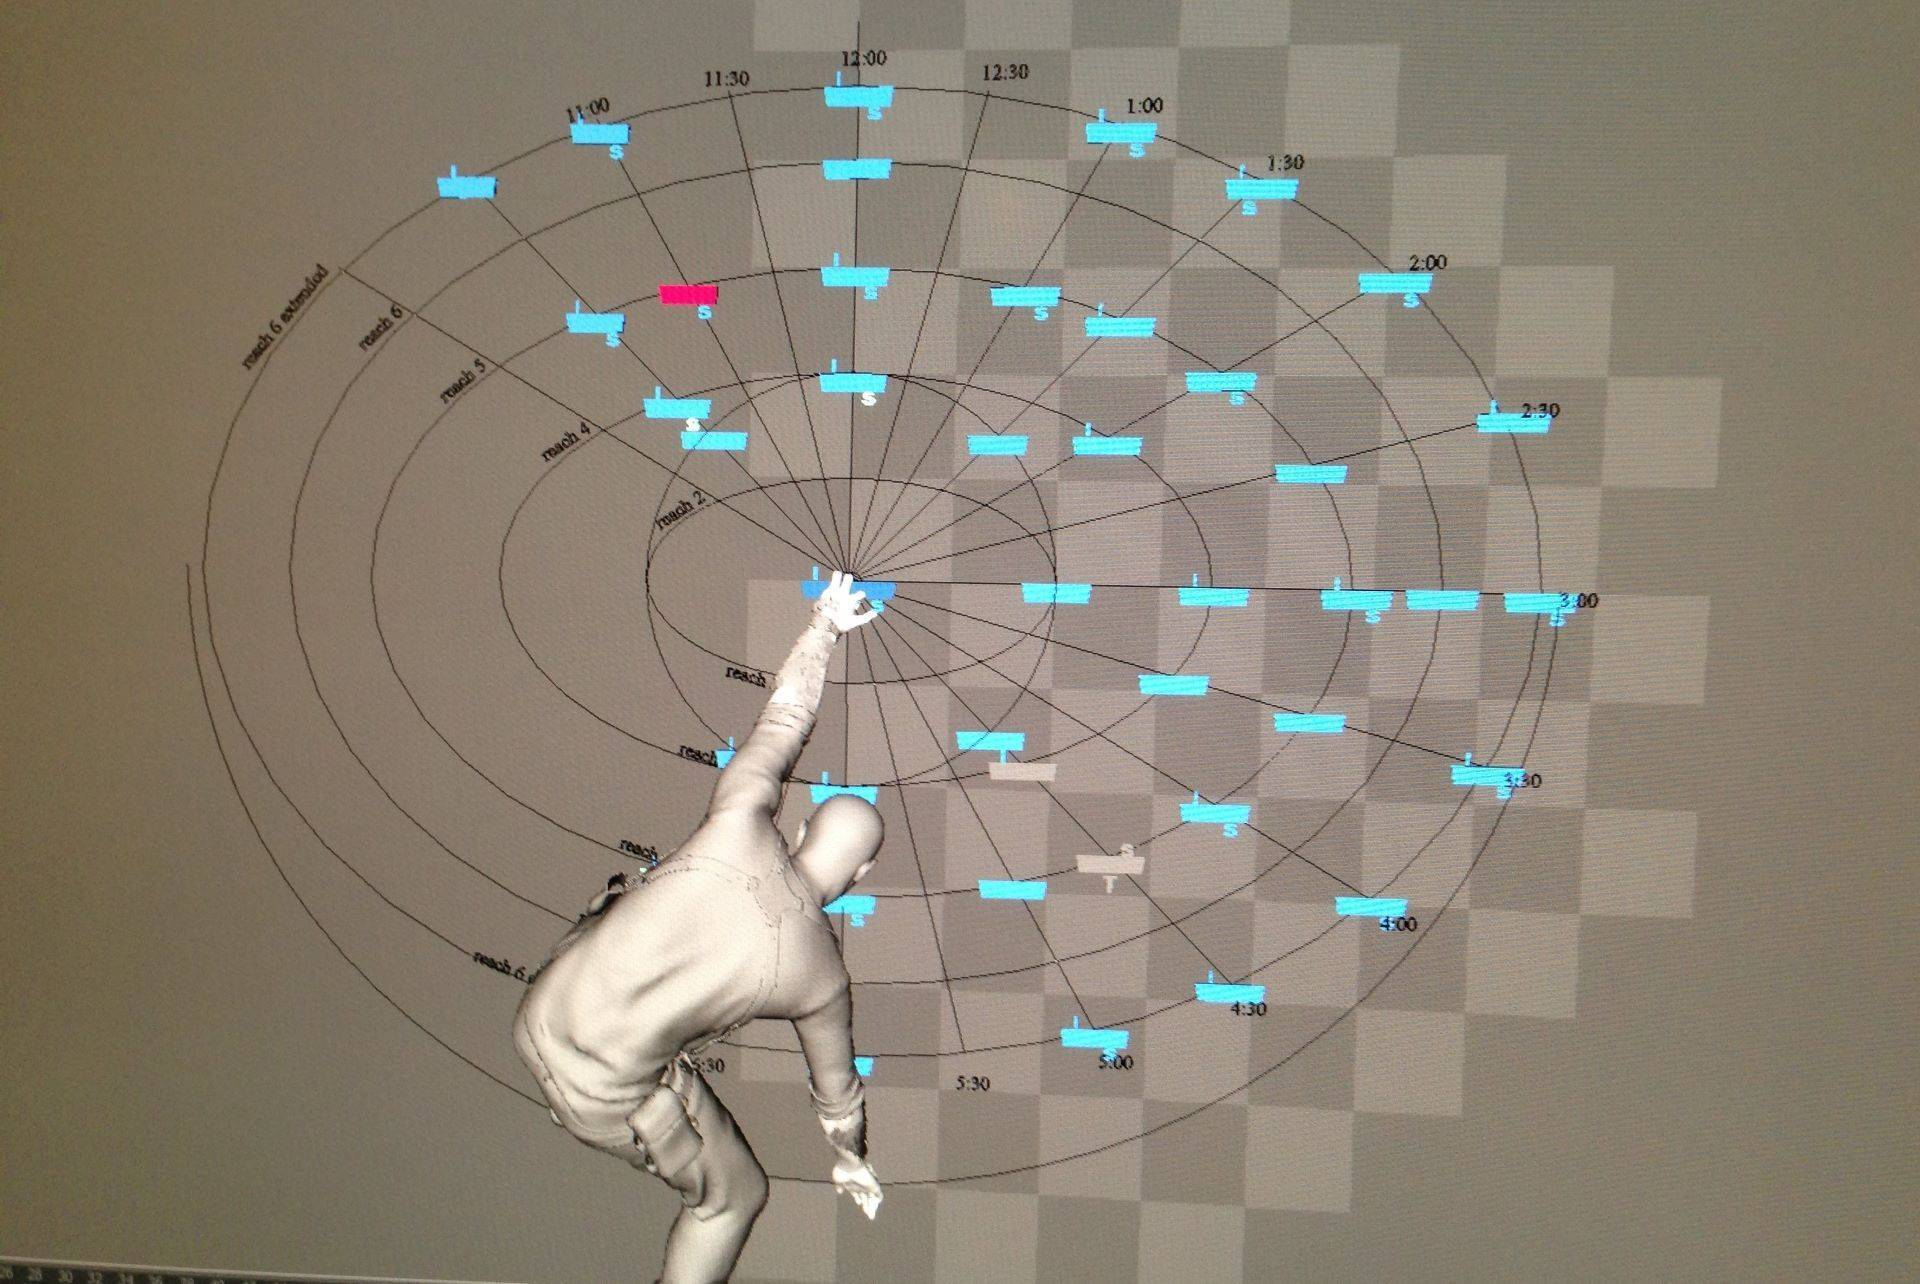
\includegraphics[scale=0.125]{climbing-reach-diagram.jpg}
\caption{Uncharted 4 (2016) uses an inverse kinematic solver to create dynamic climbing mechanics that react to the world around them based on player input.}
\end{figure}


\section{Technical Background}
At its most basic, an inverse kinematic (or IK) solver positions a system of joints such that the final joint, or end effector, is as close as possible to an input target position. In doing so, the chosen IK algorithm calculates the position and rotation of each joint from the anchored root to the final end effector. The majority of IK algorithms utilized in modern media are iterative. As such, in real time applications like game development a lightweight semi-realistic algorithm is preferable to a complex but highly precise implementation \cite{litReview}\cite{ZucconiIK}.

To this end, when choosing an IK algorithm for a character animator there are a few key factors to consider. The first is simply the speed of the algorithm. When using IK in games the algorithm will be run at best one time per frame (assuming an acceptable solution is found on the first iteration). An IK algorithm used for games needs to solve in under 16 ms at the absolute slowest. This assumes a game running at 60 frames per second and no other significant weight on the system. The second key factor is iterative efficiency. As previously stated, IK algorithms will solve sequential arrangements of joints until the target is within an acceptable tolerance range. The efficiency of an IK solver relies not only on how fast each iteration is but also on how many iterations are needed to solve the system \cite{litReview}\cite{baseFABRIK}. Fewer iterations leads to a faster solution which in turn means an efficient and reliable algorithm. The final factor in choosing an IK algorithm is realism. IK solvers used to animate game models need to create realistic poses in order to offer a true alternative to traditional keyframe animation. Meaning, the algorithm must move joints from one target position to another smoothly while also maintaining realistic joint angles and positions. Because of this, many fast and iteratively efficient algorithms are not suitable for game development purposes. 

There are countless IK algorithms, all with their own benefits and drawbacks within the aforementioned factors. The process of selecting an algorithm for use in a game engine starts by trimming down the set of available algorithms by considering what actions the character controller will need to perform. \textcite{spore} for example created a particle based IK system for the game Spore (2008) to project singular predefined animations like dancing and fighting onto the innumerable creatures that the player creates and modifies as part of the core gameplay loop. While particle IK systems can be fine tuned for just about any use case, the complexity of implementing this algorithm far outweighs the potential benefits when only animating a humanoid controller. 

Another factor that makes it easy to trim several well researched algorithms from the search is the common use of complex matrix calculations. These can compound quickly in systems with higher degrees of freedom such as multi-end effector system or long joint chains. This rules out the versatile Physics based Newtonian methods as well as Jacobian solvers that are popular in the field of Robotics for their accuracy and reliability \cite{newtonian}\cite{jacobianSingularity}. Despite being some of the most researched and reliable methods both of these families of algorithms utilize a number of matrix transformations and calculations to achieve their precision results. This makes them unnecessary for a lightweight character animator \cite{litReview}.

Cyclic Coordinate Descent is a noteworthy algorithm that was a popular choice for game developers in the 2000s to animate characters and limbs. It is a heuristics based forward kinematic solver that rolls and unrolls a limb to iterate towards a solution by minimizing the distance between the end effector and target\cite{CCDBlog}. CCD converges quickly, is lightweight, and has been implemented to great effect in games like Shadow of the Colossus (2005) for both humanoid and creature animation systems \cite{ShadowofC}. CCD does have some drawbacks however. Firstly, it requires significant and expensive alteration to extend well from single joint chains to systems with multiple end effectors. Second, it can suffer from singularity issues making certian target positions unreachable. Finally, CCD can produce unrealistic poses due to the rolling and unrolling movements the algorithm uses to reach its target. For these reasons CCD is often blended with keyframe animations, extending the predefined motions to changing scenarios like idling on uneven ground or pointing a finger at moving targets \cite{baseFABRIK} \cite{CCDpaper}. Cyclic Coordinate Descent is a powerful IK solver but in recent years more flexible heuristic solvers have become more common.

FABRIK, or Forwards And Backwards Inverse Kinematics, is one of the most utilized IK solvers in the modern day. FABRIK solves joint systems by treating joint-bone relationships into points connected by vectors of constant length. This makes it simple to implement, computationally cheap, and suitable for most applications where the believability of poses is more important that the precision of the movement to get there \cite{FABRIKoptimized}. FABRIK converges quickly and creates believable poses that consider current joint positions to solve with minimal adjustments \cite{baseFABRIK}. Additionally it is easy to expand and constrain FABRIK to create complex models with multiple end effectors like a human skeleton \cite{extendFABRIK}. This makes it ideal for animation and has led to it being used in countless games from both large and small developers.

FABRIK process a limb as a series of joints $P_1...P_i$ where each joint stores its own position and rotation. Additionally, joints must remain at a fixed distance or bone length $L$. It should be noted that for more complex systems each joint may hold a different bone length represented by $L_1...L_{i-1}$; However, for the sake of simplicity a uniform $L$ value will be assumed. Finally, the root joint $P_1$ needs a root position, $R$, and the end effector $P_i$ needs a target position, $T$.

Given these inputs, FABRIK solves the inverse kinematics problem as a two step process. Firstly, in the backward reaching step the position of the end effector $P_i$ is set equal to the target position $T$. Then, by calculating the difference in positions between the next joint in the chain, $P_{i-1}$, and $P_i$'s new position, a vector pointing from $P_i$ towards $P_{i-1}$ is found and normalized to a directional vector $D_{i-1}$. Finally, Multiplying $D_{i-1}$ by the bone length $L$ gives the new position for $P_{i-1}$ that preserves the constant bone length. With $P_{i-1}$ adjusted to its new position the process repeats. The vector from $P_{i-1}$ to $P_{i-2}$ is found, normalized, and scaled to $L$ before moving $P_{i-2}$ to its new position. This process continues down the limb until the root is reached. The forward reaching pass follows the same process but in reverse order. $P_1$ is moved back to the root position before solving forwards through each joint until the end effector is reached. This cycle then iterates through the forward and backward steps until the distance from end effector to target is below the chosen tolorance range (ex. 0.1) \cite{baseFABRIK}. Figure 1 illustrates the start of a backward step.

\begin{figure}
\begin{subfigure}{.4\textwidth}
  \centering
    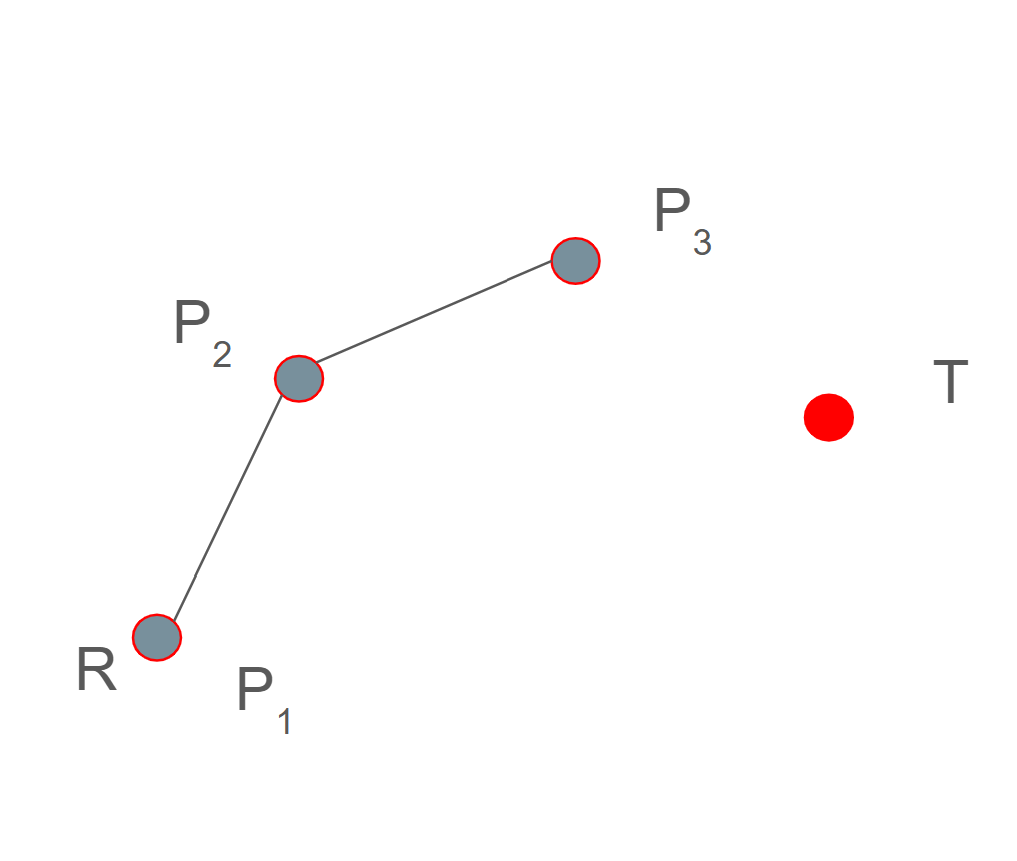
\includegraphics[scale=0.4]{start.png}  
    \caption{Initial state of the joint structure}
  \label{fig:sfig1}
\end{subfigure}
\begin{subfigure}{.4\textwidth}
  \centering
    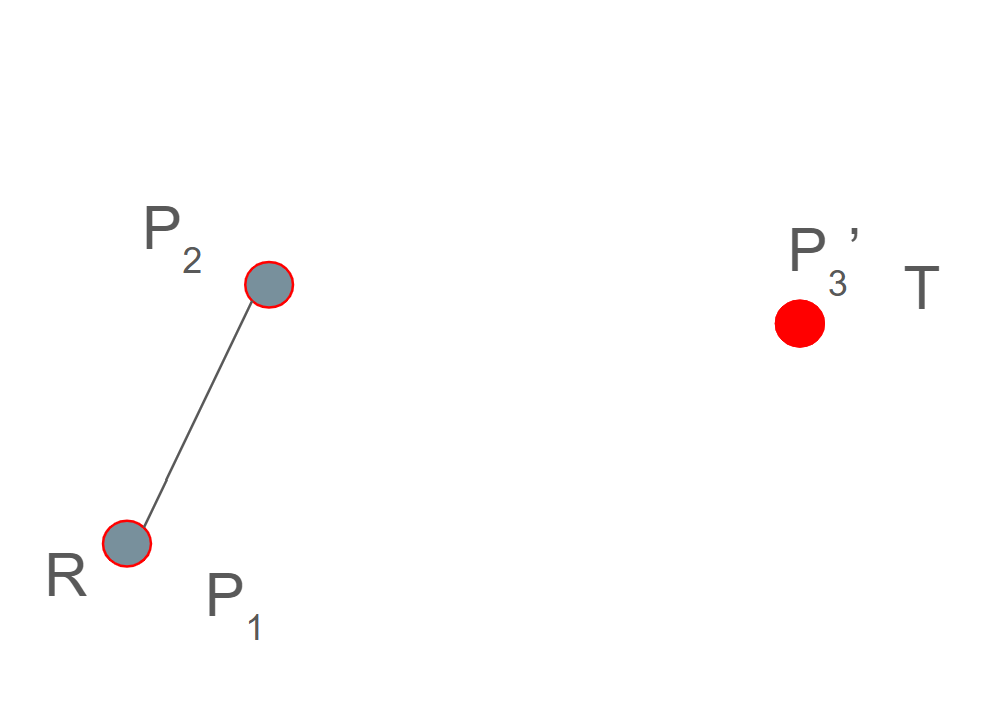
\includegraphics[scale=0.4]{step1real.png}  
    \caption{End effector is moved to the target position}
  \label{fig:sfig2}
\end{subfigure}
\begin{subfigure}{.4\textwidth}
  \centering
    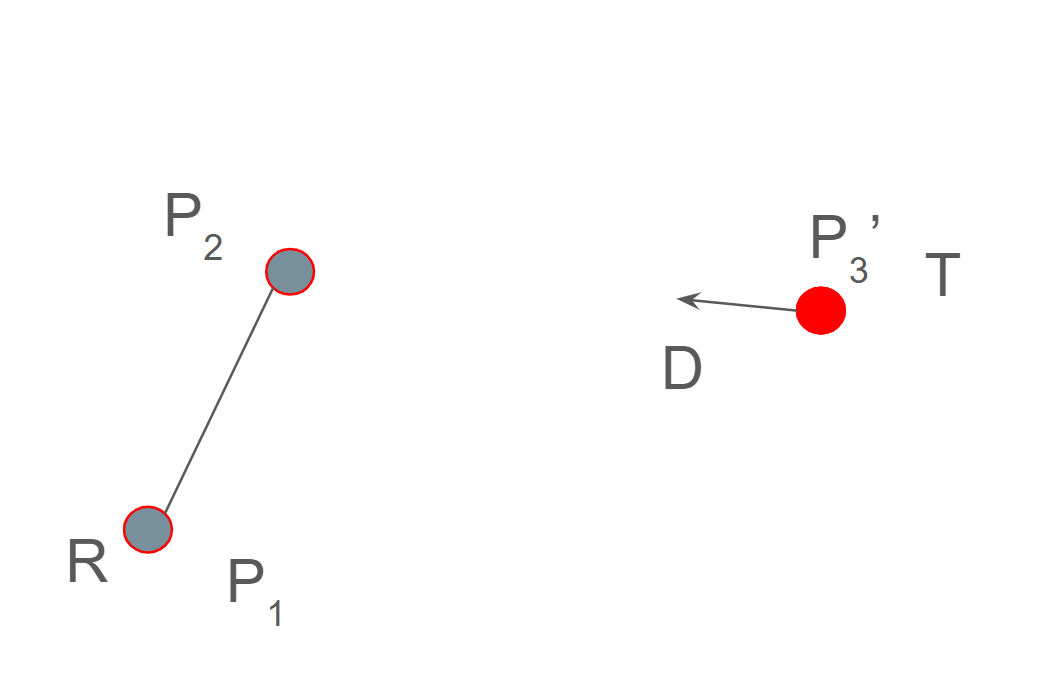
\includegraphics[scale=0.4]{step2.png}  
    \caption{direction vector $D$ is found from $P_i$ to $P_{i-1}$}
  \label{fig:sfig3}
\end{subfigure}
\begin{subfigure}{.4\textwidth}
  \centering
    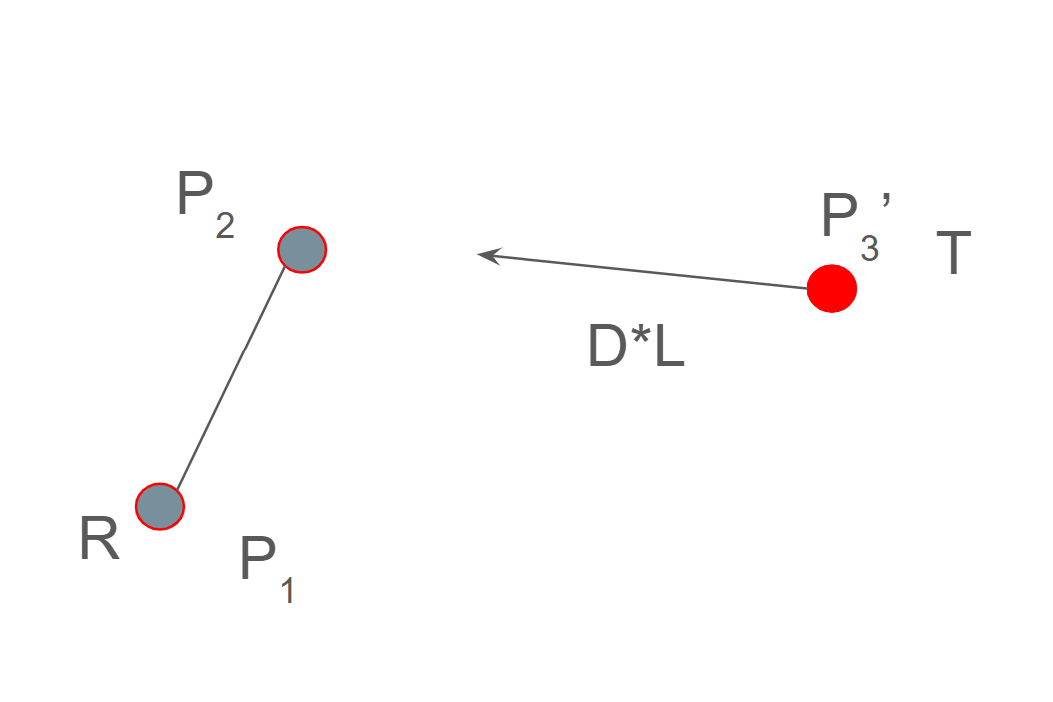
\includegraphics[scale=0.4]{step3.png}  
    \caption{D is multiplied by bone length $L$}
  \label{fig:sfig4}
\end{subfigure}
\begin{subfigure}{.4\textwidth}
  \centering
    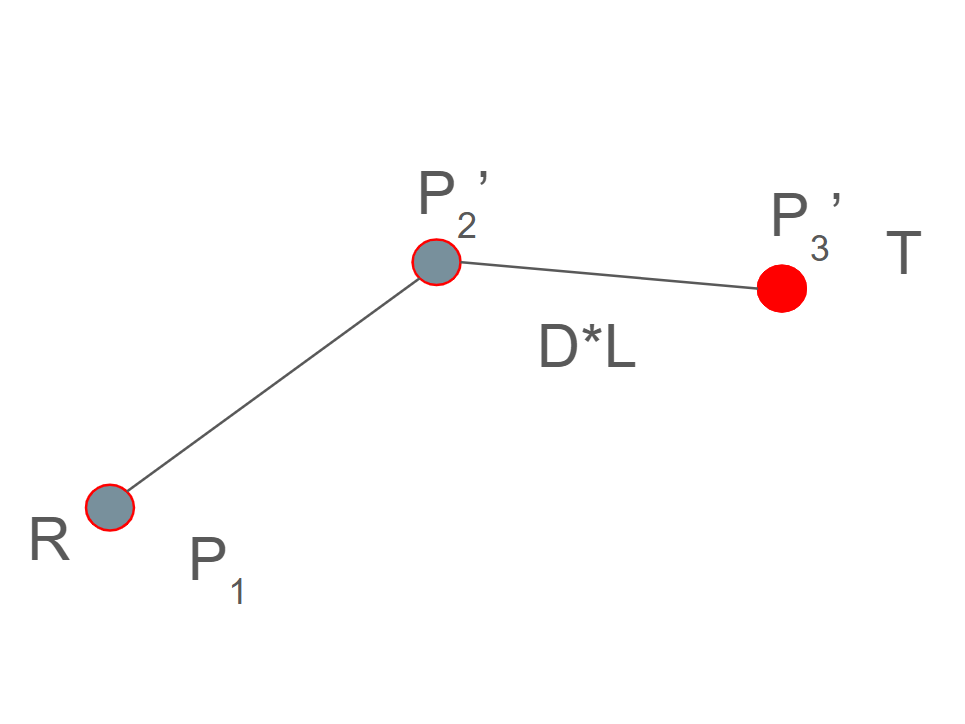
\includegraphics[scale=0.4]{step4.png}  
    \caption{$P_{i-1}$ moves to the end of the lengthened $D$ vector}
  \label{fig:sfig5}
\end{subfigure}
\caption{This diagram shows the first backward step of the FABRIK algorithm. This would be run for each joint before being reversed and run as the forward step.}
\label{fig:fig}
\end{figure}




\section{Prior Work}
Forwards and Backwards Inverse Kinematics was first created by \textcite{baseFABRIK}. Aristidou's original study demonstrated FABRIK’s ability to produce natural looking poses for a variety models. Additionally, the study posed a framework for constraining joints using a series of vector projections and transformations to restrict poses and create more realistic models \cite{extendFABRIK} \cite{quadruped}. Aristidou and Lasenby’s data shows that FABRIK vastly outperforms the speed and number of necessary iterations of CCD, Jacobian, DLS, and other popular solvers in both single and multiple end effector tests. 

\textcite{extendFABRIK}, Aristidou and Lasenby’s supplementary research on constrained FABRIK models, explores performance in edge cases as well as the feasibility of implementing realistic biological joints. They were able to implement basic pivot, ball and socket, and hinge joints using their unmodified constraint model. However, condyloid, saddle, and plane joints required alterations to the algorithm to allow inter-joint distances to fluctuate with movement. This research makes their vector based rotational model a desirable option compared to other IK constraint schemes like quaternion rotation constraints or Polar coordinate restrictions \cite{CCDpaper}\cite{CCDBlog}. It’s worth noting that the infeasible joint types that require alterations can be largely ignored in a game development environment as a convincing product can be made with only pivot, ball and socket, and hinge joints when constrained properly. 


\section{Model Design Methods}

The base FABRIK algorithm provides a foundation that can easily be applied to 3D objects to create modular joint chains. The focus of this research is a model built in the Unity 3D game engine. Unity allows each joint to exist as its own object that is then positioned by a single parent body object that runs the FABRIK solving script. For ease in up-scaling and management, each joint object inherits a base FABRIK joint class that stores unique information like bone length and parent joint object references. This is helpful when adding joint types and constraints later on. All joints are referenced and controlled by the central body script that organizes and solves the chain using the modified FABRIK algorithm. Figure 2 shows this basic form of 3D FABRIK running on a single end effector chain in Unity. 


\begin{figure}[h]
\centering
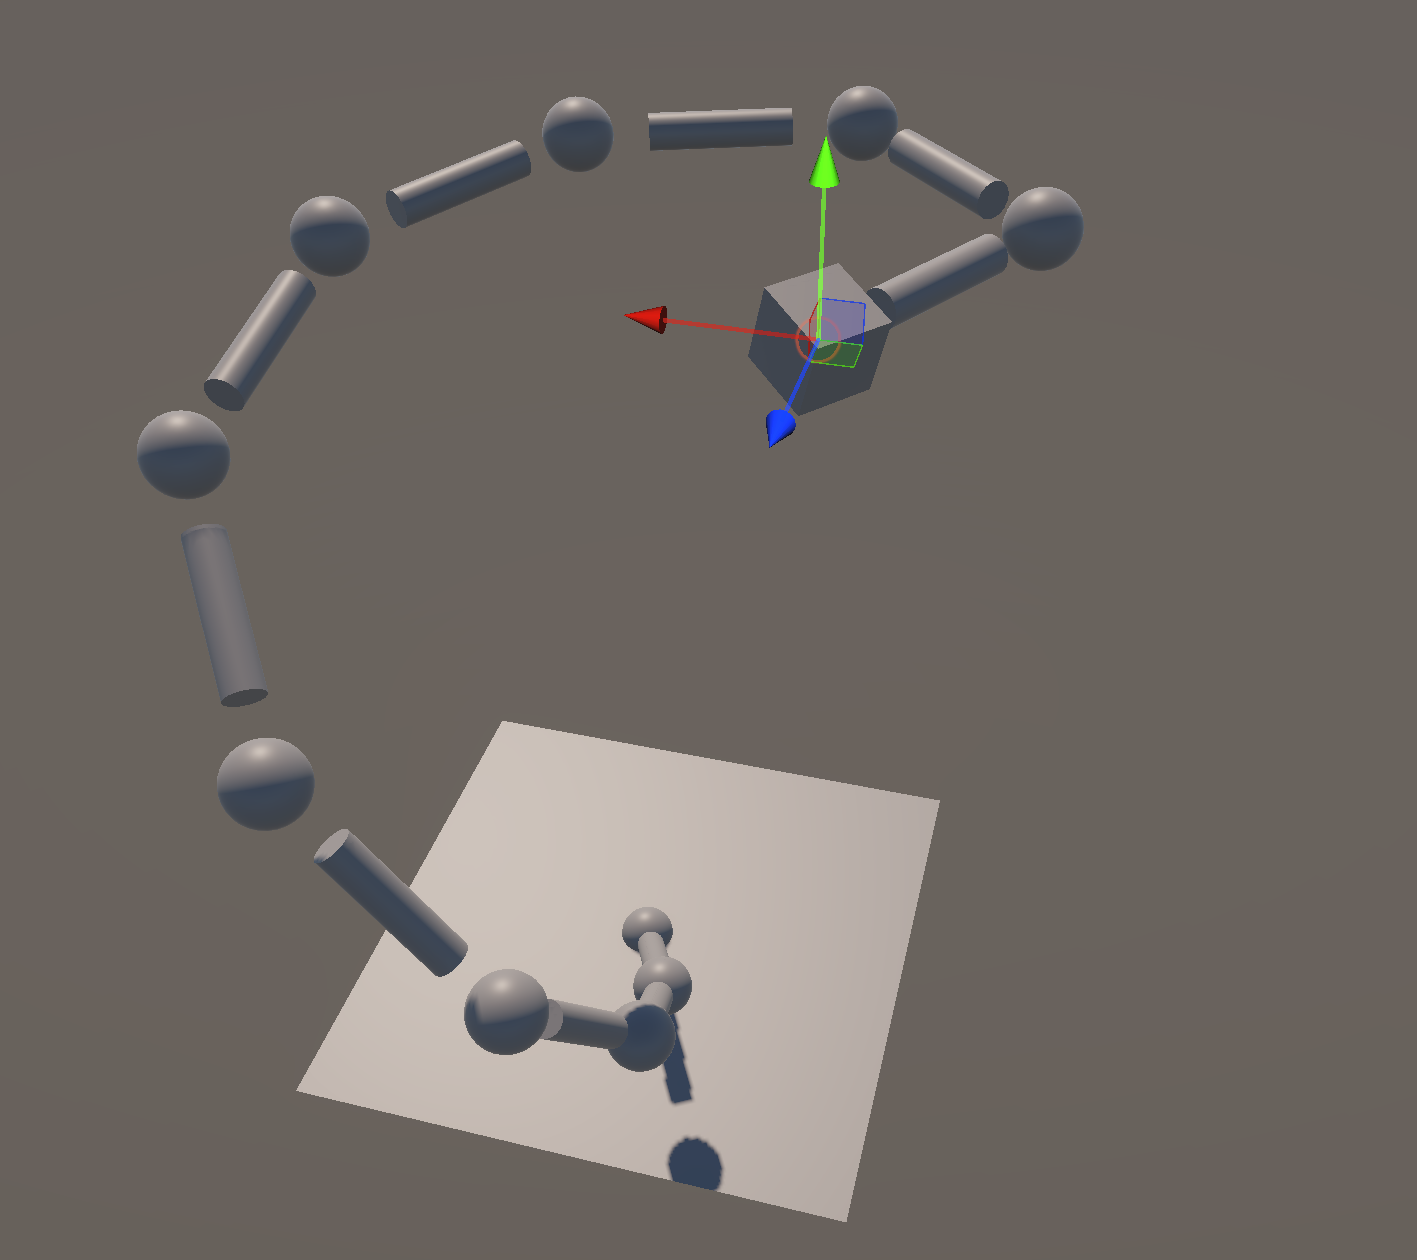
\includegraphics[scale=0.45]{FABRIK3D2.png}
\caption{A single end-effector model showcasing organic movement and poses using the unconstrained FABRIK algorithm. Created in Unity 3D}
\end{figure}

In order to create a complex skeletal model, both the solver algorithm and joint objects need to support structures with multiple end effectors and joint connections. Adapting both of these is fairly simple. First, joints belonging to multiple chains are identified and classified as subbases. For this model's simplified humanoid skeleton these subbases are the upper chest and hip joints. Subbase rotation must remain independent of the joint systems they are connected to. This can be accomplished by checking the first and last joint of each chain before updating their rotation. If any of these joints are subbases their rotation is set to a constant value instead of facing the joint ahead of it in the chain. In this case, the subbases are set to face the vector (0,0,1) which defines the forward direction in the local space of the parent body object. Subbase rotation can modified algorithmically for specific use cases. For example the upper chest can be safely assumed to face orthogonally to a vector connecting the two shoulder joints, allowing the shoulders and hips to twist separately when following detailed animations. However, for this use case subbase direction was held constant. Once subbases are established each chain can be solved from the outside in. Meaning the arms, legs, and neck are solved independently before finally solving the spine and completing the skeleton \cite{extendFABRIK}. 

\begin{figure}[h]
\centering
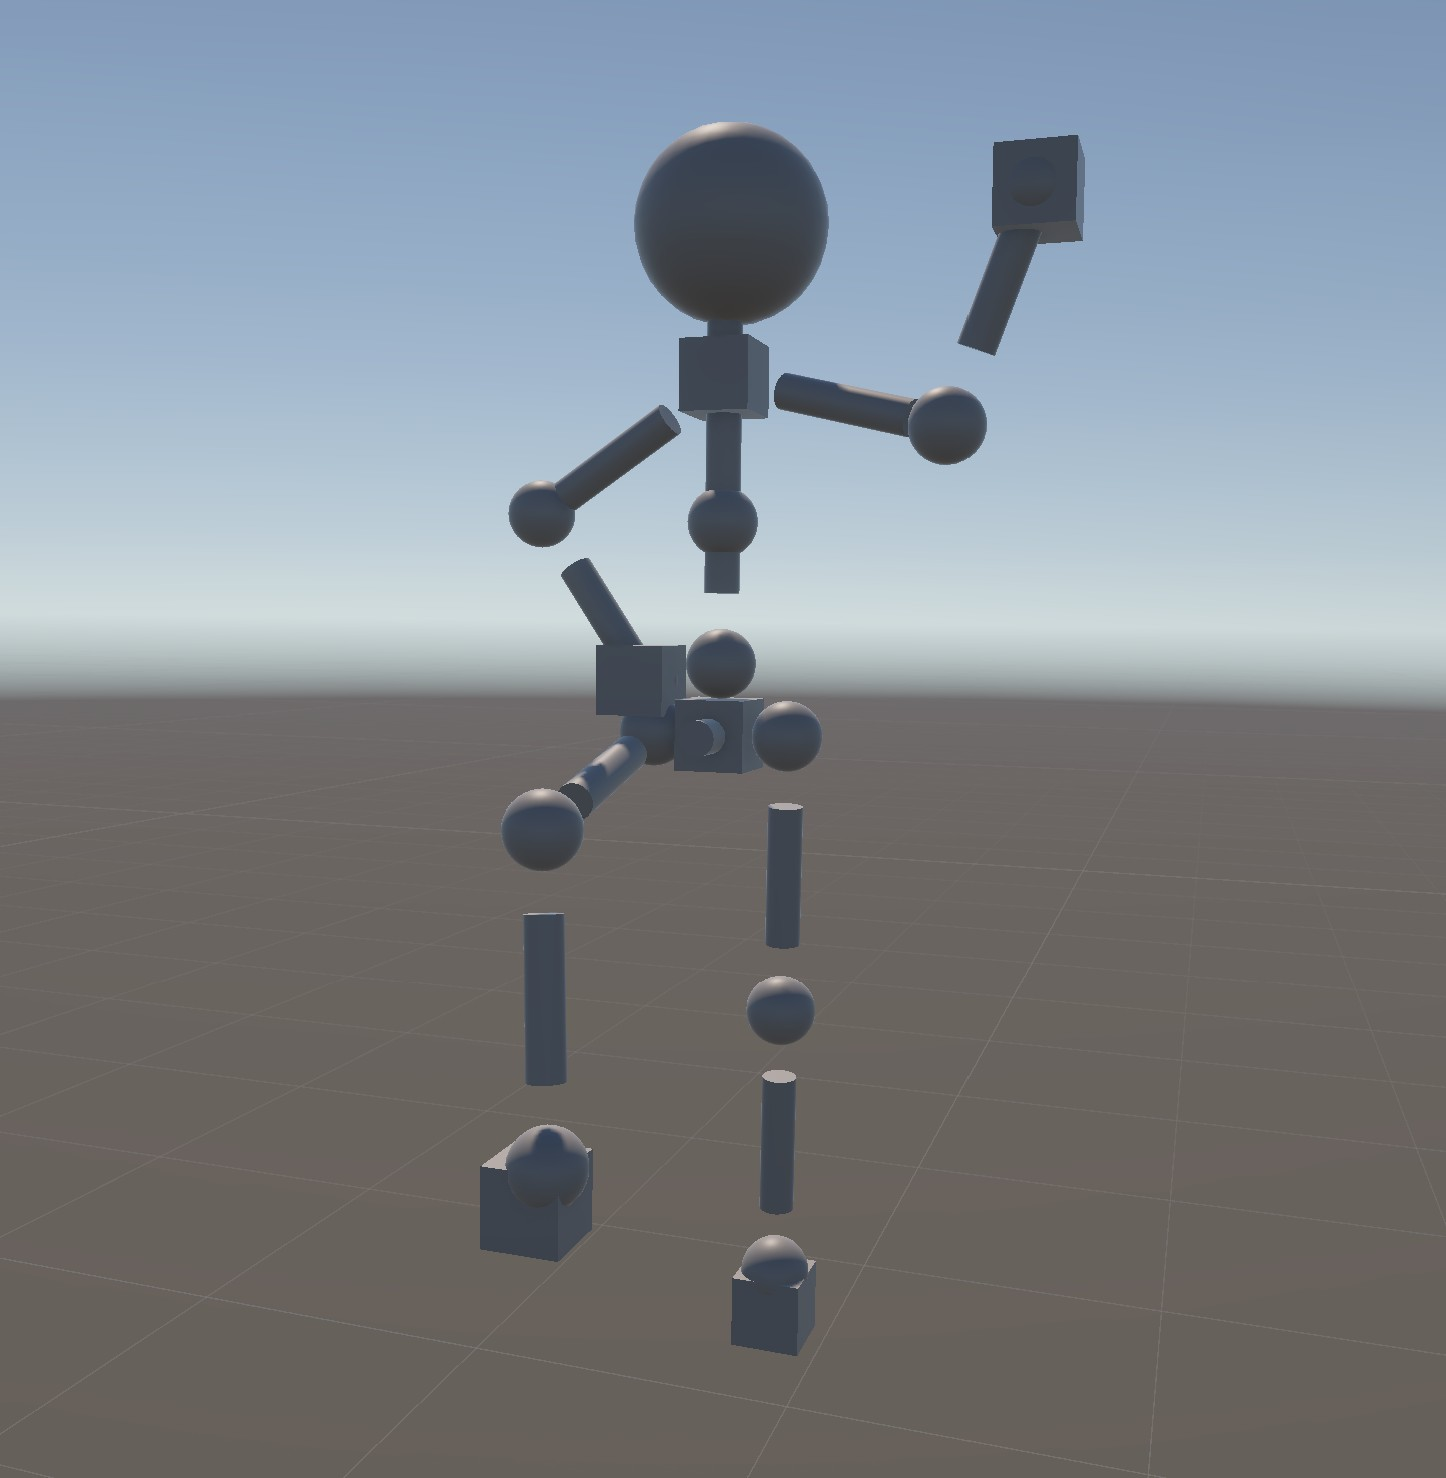
\includegraphics[scale=0.5]{Poster2.jpg}
\caption{A constrained skeletal model in a solved position. Created in Unity 3D}
\end{figure}

With the skeletal object assembled, each joint must now be categorized and constrained to mimic human range of motion. This process starts by creating specialized ball and socket, hinge, and pivot joint classes that inherit the base FABRIK joint class but restrict valid target positions before adjusting the joint on the forward pass. Regardless of the type of joint, the process of constraining its position utilizes the same base algorithm with minor adjustments to create unique ranges of motion. Constraining positions in 3D is normally quite complicated and expensive, utilizing either Euler angles, which suffer from gimbal lock, or Quaternions that become difficult to control when ranges of motion beyond a regular spherical sector. Instead, the 3D problem can be converted into a 2D problem by projecting both the joint and its target onto a 2D plane, solving the constraint problem using a series of line intercept calculations, and finally translating back into 3D \cite{baseFABRIK}\cite{CGjointStructure}.

 The constraint process begins by setting up the 2D problem and checking if constraints are needed for the given target. Joint constraints are applied on the forward pass which allows the system to build on top of joints that have already been constrained and solved. This starts by taking a solved joint $P_i$ and a our target position, $T$, for the next joint $P_{i+1}$. Both the solved joint position and the target are projected onto the 2D plane that is orthogonal to a chosen constraint dimension (either X, Y, or Z). This creates a 2D projected parent joint, $L$, and a projected target, $O$, both of which are then translated such that $L$ is located at the origin of the 2D plane. From there 4 constraint lines are defined, $c_1$...$c_4$, each of which represents the extent of motion in a particular quadrant of the 2D plane. Together they enclose the allowed range of motion of the joint $P_i$. If $O$ is within this enclosed region then there is no need to constrain $T$ and the algorithm can move forward using the original target. However, if $O$ is outside of the enclosed range then it must be adjusted to the closest point within the constraint boundaries. To constrain an out of bounds target the vector connecting $L$ and $O$ must first be found. Finding the intersection between this vector and the constraint boundary for whichever quadrant $O$ is in gives the closest point inside the constraints $O'$. $O'$ gives an adjusted target position in 2 of 3 dimensions which means there are only 2 possible values for the third dimension that conserve constant joint length, one positive and one negative. For some joints, like shoulders, that are restricted to a single side of the body choosing either the positive or negative value works best. For others choosing whichever value ends up closest to the target is also an effective solution. With all position values found the new target, $P_i$ is then added to $T'$ bringing it to the final constrained target position.

 The base constraint process creates a ball and socket joint but it can be easily converted into a pivot joint by setting all constraint lines to intercept at the origin, completely restricting movement while still allowing rotation. Hinge joints are a little more complex but utilize the same ideas. Projecting to a 2D plane removes one degree of freedom from the system which effectively creates the most basic hinge joint possible. By normalizing $L \rightarrow O$ and measuring the angle between the line and (0,1) theta can be found and restricted to acceptable values \cite{extendFABRIK}.

 It is worth noting that the constraint method explained above must be centered on one of the X, Y or Z axes. However, this can be adjusted by measuring the rotational offset from the constraint axis to $P_i$'s rotation as a quaternion, $Q$. Multiplying $Q$ and $T$ removes $P_i$'s rotation temporarily allowing the constraint intersections to be measured on the same 2D coordinate system. After constraining,  $Q^{-1}$ and $T'$ are multiplied which re-applies $P_i$'s rotation allowing $P_{i+1}$ to be constrained with regards to $P_i$'s local X, Y, or Z axes but maintain the parent joint's impact on the child joint's rotation \cite{swingTwist}\cite{Quaternions}.

 \section{Experiments}

 To measure the versatility and accuracy of the FABRIK skeletal model it was tested against motion capture data gathered using Sony Mocopi sensors. Mocopi's customization capabilities allowed test data to be recorded using sensors placed on the body to mimic the locations of the targets that the FABRIK model uses to update joints. 30-60 second animation segments were recorded, uploaded to Unity, and applied to a standard humanoid rig. The FABRIK targets were then set to follow the wrists, arms, head, chest, and hips of the motion capture armature while measuring the joint offsets between the two models. This allowed the measurement of the FABRIK model's ability to mimic human movement while also measuring the tuning of the joint constraints. A perfectly tuned model able to follow closely from frame to frame would see average offsets at or under the set tolerance range of 0.1 Unity meters \cite{FABRIKMocap}\cite{benchmarkGit}. 

 This same experiment was then repeated again but using motion capture data gathered with extra sensors at intermediate joints. In this case extra sensors were placed at the upper arms and upper legs to allow better tracking of knee and elbow joints. Using this data the same tracking test was run with additional offset tracking for the elbow and knee joints. While tracking end effector offsets measures how well the FABRIK model can reach it's target, measuring intermediate joint offsets gives a better look at how well the model can mimic human poses and movements algorithmically. 

 Before discussing the results of these tests it is important to note that the skeletal model animated with motion capture is not equivalent to the skeleton built by the FABRIK model. The motion capture armature has extra joints throughout the spine, neck, and chest which makes it difficult to precisely measure and mimic the joint lengths of the model when constructing the FABRIK skeleton. Additionally, the flexibility of the human body can only be estimated by the linear constraints used in this model. As such we expected to see larger offsets in the chest and neck joints as well as the intermediate joints that would more severely be affected by model posture and cascading constraint error.

 \begin{figure}[h]
\centering
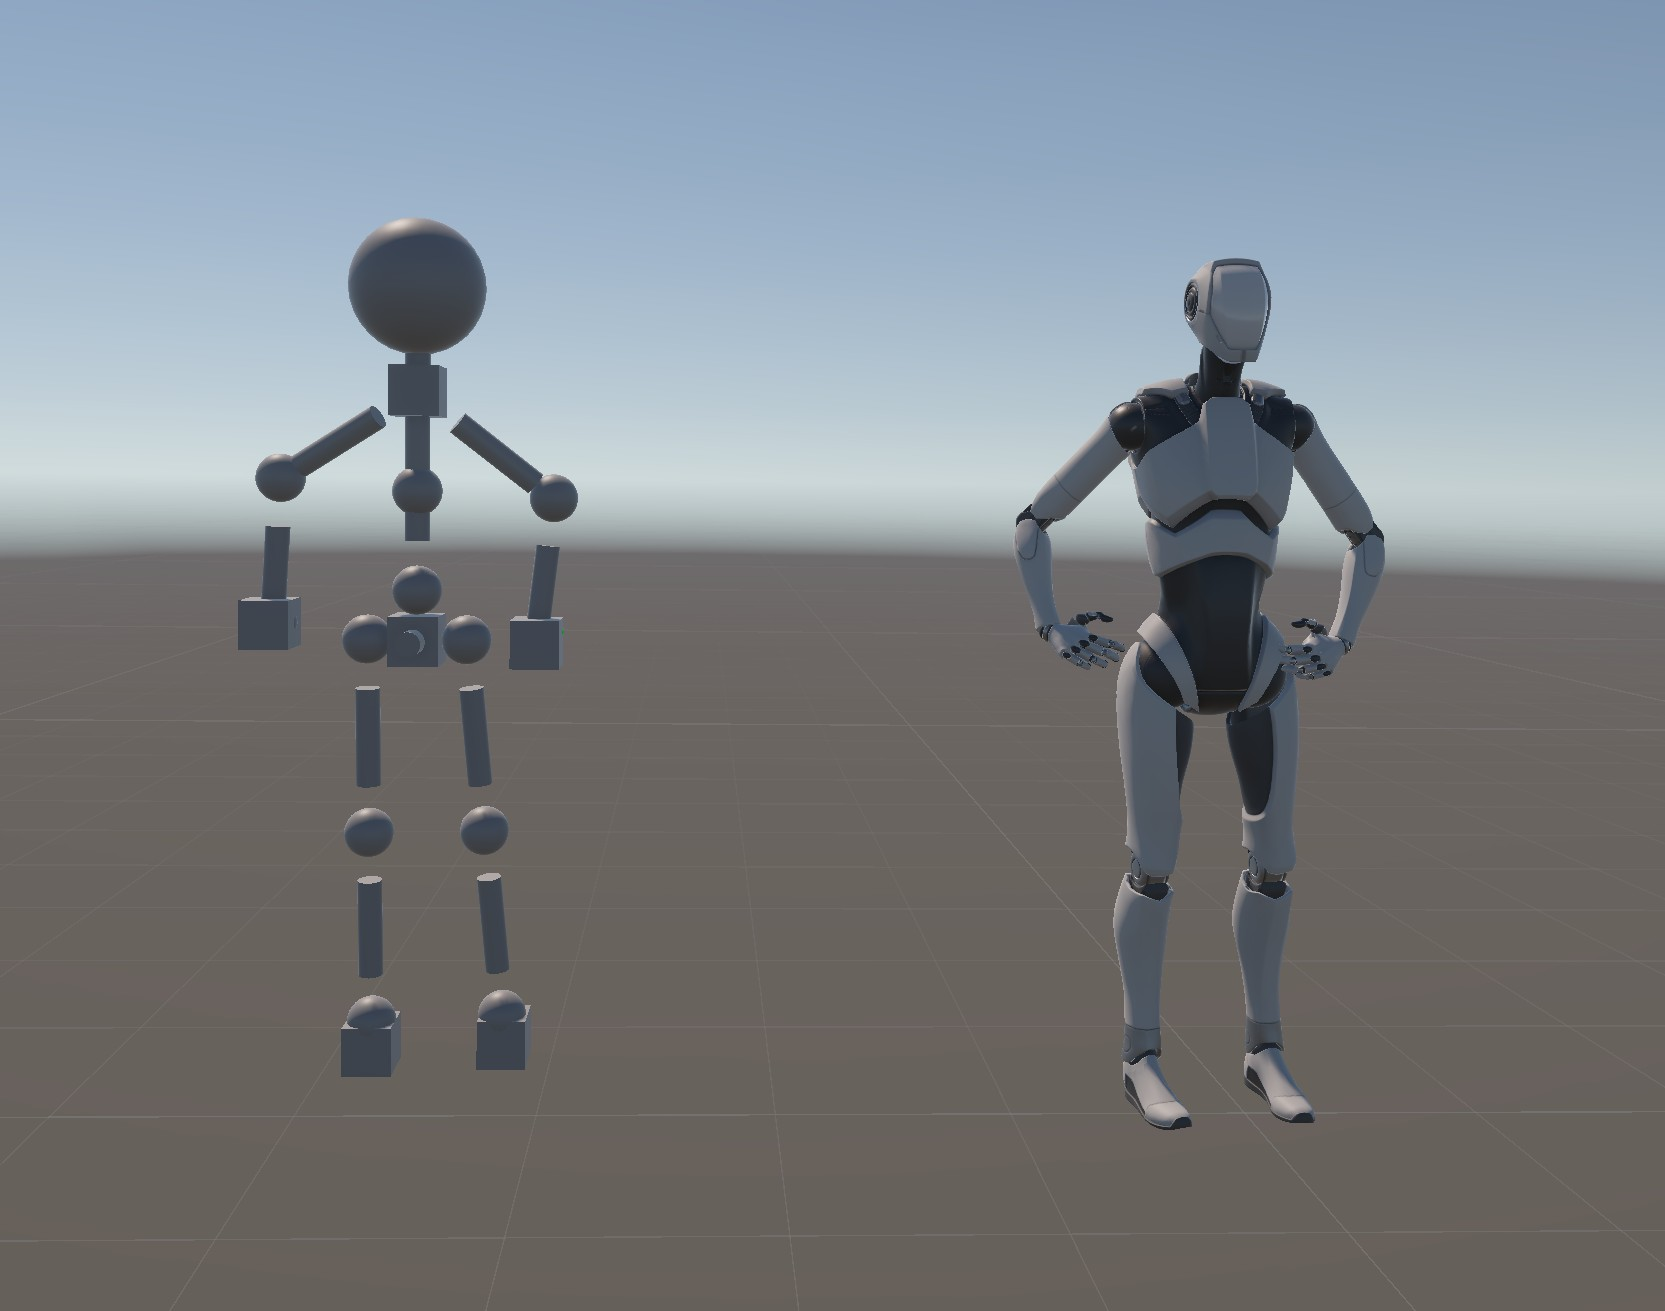
\includegraphics[scale=0.45]{Poster1.jpg}
\caption{FABRIK skeletal model (left) matching the pose of a motion capture animated model (right).}
\end{figure}


 \section{Results}

 In the first test, the FABRIK model was able to follow the motion capture data closely. The wrists and ankles remained near their tolerance range of 0.1 Unity meters throughout the experiment with wrists averaging 0.4 Unity meters and the ankles averaging 0.3 over the course of the animation. For reference the entire model is 15.5 Unity meters tall meaning the end effectors stayed well within an acceptable range given the constraints on the model. The head and chest joints were also able to follow the data though not as closely; however, given the aforementioned model differences, FABRIK was able to effectively translate from from motion capture data to procedural animation. 

 The second test showed that intermediate joints had a much harder time matching the motion capture data without the aid of an explicit target. The knee joints averaged 1.2 meters of offset while elbows averaged 1.0. This offset seemed to be caused by different rotations in early limb joints like the shoulders. This model only constrains the position of joints not the rotations. Meaning, for hinge joints like the elbows and knees it was possible to find quicker solutions with different joint positions by rotating the shoulder joints to odd angles thereby working around the set constraints to minimize overall joint movement. While the created poses were still valid within the joint constraints, they created larger offsets for intermediate joints due to the differing solutions. These results suggest that more precise constraints that address position and rotation simultaneously may be necessary to better mimic human movement. 
 

 \begin{figure}[h]
\centering
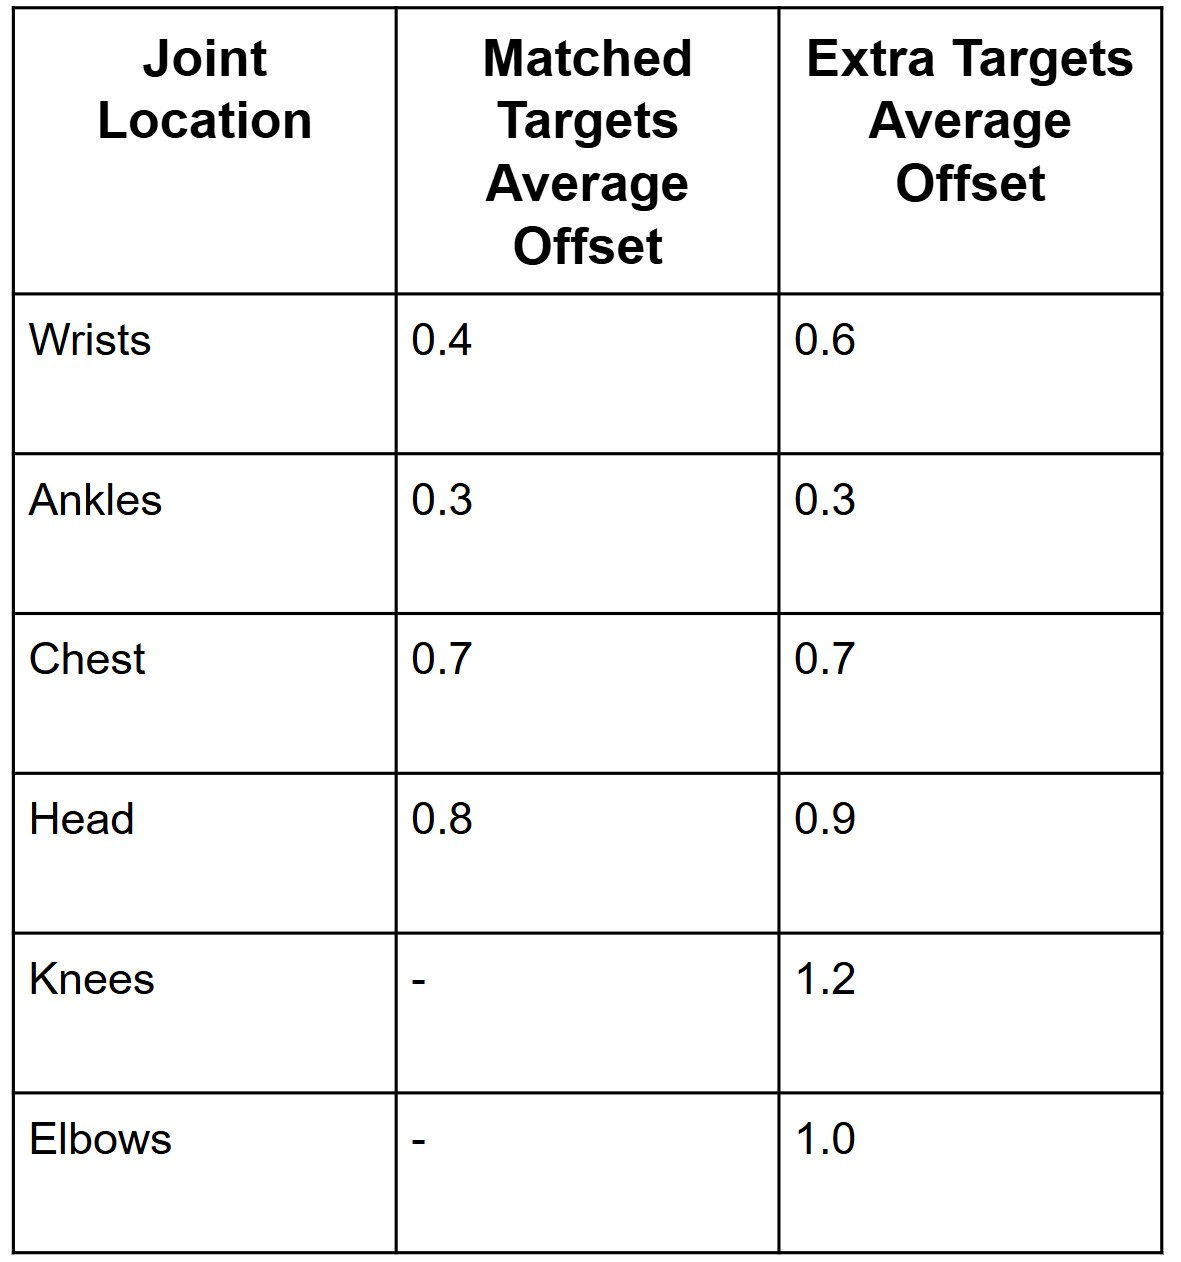
\includegraphics[scale=0.5]{table1.jpg}
\caption{Average distance from FABRIK joint placement to motion capture placement for each joint type with a motion capture sensor across two tests. For reference the FABRIK model is 15.5 Unity meters tall.}
\end{figure}






\section{Discussion}

\subsection{Ethical Considerations}

The ethical considerations of inverse kinematics are as varied as the applications. Procedural animation on its own is not a risk to security, privacy, or personal freedoms but some of its applications can raise concerns in these areas. Animated media is like all other forms of media in that it must be created and maintained responsibly. Providing easily accessible animation tools to developers does create a risk of irresponsible use; however, when considering the wide array of free animation applications available to the average consumer and the limited scope of this research it is clear that this FABRIK skeleton model does not pose any additional ethical risks.

\subsection{Code Overview and Replication Instructions}

The FABRIK skeletal model as well as the building blocks used in its creation are build in Unity 6.0. As such, downloading the game engine and opening the source files as a new project will automatically create all of the dependencies needed to recreate the results from this paper. All of the scripts, object prefabs, and other files utilized in the creation of this process are stored in the Assets folder of the Unity project files. 

Building upon these results for further research or creating a customized skeletal model may take a more in-depth understanding of how this model interfaces Unity's object oriented engine. The experimental model that this paper focuses on uses the FABRIKSolver script to organize and animate the skeleton. Skeletons that use this script or any derivative scripts must start with a empty parent 'body' object. Joint chains are then added as children of the body object such that they use the empty parent as their base world position. This lets the whole skeleton be moved as a single body which is essential if utilizing any form of character movement script. It is also important that the joints are not made children of one another. While this is a common technique for some animation rigs, this solver manipulates all joints in world space independently of their parent objects. Parenting the joints to one another will cause the movement of one joint to move all its children in the same manner. FABRIK builds each limb one joint at a time, so moving unsolved joints through parenting leads to inaccurate solutions. 

The FABRIKSolver script's serialized field variables allow it to store references to each joint's game object in order to manipulate their transforms at runtime. These references are organized into arrays for each limb so each array can be iterated during a forwards and backwards step to solve a single limb at a time. The solving process then runs the FABRIK algorithm on each of these arrays in a set order until a solved position is reached. 

Each joint game object has a FABRIK joint script that holds unique data each joint's bone length, constraint ranges, constraint axis, and a 'sidedness' variable. While most of these fields are self explanatory, sidedness is a bit more complicated. When a constrained joint is projected into 2D and solved it leaves 2 possible values for the 3rd Projected dimension that preserve the joints constant length. Because the constraint process translates the joint in question to the origin of the 2D plane we are also able to assume it is at the origin of the 3rd dimension's axis. As such, one of these values will always be positive and one will always be negative (excluding a zero value). Sidedness collapses this choice and picks either the positive or negative side of the 3rd dimension. This is eliminates positional snapping between the two possibilities and allows mirrored joints like shoulders to be reused on the other side of the body. Constrained joints inherit from a base joint class and override the empty constraint function with their specific algorithm. This structure allows each joint to be edited at runtime allowing the skeleton to be fine tuned with ease. 

All of the scripts that make up this project are built to be flexible building blocks that can be utilized to create any kind of skeleton. By adapting the FABRIKSolver script all joint, constraint, and utility scripts can be recycled to form the animation foundation for a wide variety of projects. 


\subsection{Conclusion}


 While the FABRIK skeleton model wasn't always able to match the motion capture data, the ways in which the model solved the given animations were more often than not still possible human-like pose solutions for the target arrangement. This suggests a need for encoding movement preferences in the algorithm to supplement joint constraints. As an example, most people prefer to keep their elbows facing downwards or outwards and away from the body even though equivalent movements could be enacted with elbows pointed inwards or upwards. \textcite{spore} utilized an artificial tension system to give tendon-like assistance when solving for joint configurations that may be a helpful aid to FABRIK's constraint process. Other methods like preserving minimum angles in limbs may also help in this process but may be more effective if utilized in the manipulation of the targets rather than the solving of the system. 

 It is also worth noting that some of the choices made to simplify this implementation of FABRIK  may have contributed to the higher offset values. Firstly this implementation utilized linear equations to define constraint boundaries because it allowed their definition using only X and Y intercepts. This streamlined the process of creating and adjusting unique joints as well as finding intercepts but leads to sharp angles at quadrant edges and restricts the complexity of joint movement ranges. These could be replaced with polynomial constraints to better define realistic joint movement boundaries.

 Another contributing factor to model error was the lack of twisting rotational constraints. The process of translating world axis constraints to a local parent joint axis greatly increases the freedom of the model to find solutions but also allows the circumnavigation of positional joint constraints by twisting the parent joint until a closer (but less realistic) solution is found. In the experimental model the rotation of a (non-subbase) joint was decided exclusively by the position of a child joint so that the bone visual indicator was placed correctly. If this model was used to animate a more traditional armature then this dependency could be removed and rotation could be constrained by isolating the swing and twist components of Unity's quaternion rotations and limiting the twist angle of each joint based on anatomical limits \cite{swingTwist}.
 
 FABRIK armatures can give creative and functional freedom to small game developers and animation studios that need to expand beyond traditional key frame animation workflows to keep up with time limits and consumer expectations. With further research into constraining methods this implementation could be applied to create a versatile joint tool-set usable in any number of configurations for a wide variety of projects. 
    



This section will demonstrate that you have thought through the basics of how your code will work. You should include a diagram of the overall data flow of your program, including what the inputs and outputs of each component will be, and how they will be represented.

 

\printbibliography

\end{document}
